\begin{frame}{Fitting of invariant masses}
  \begin{itemize}
  \item $K^- d\rightarrow (\pi^{\pm}\Sigma^{\mp})_{backwoard} n_{forward}$ (Signal)
  \item $K^- d\rightarrow K^{0} n n$ (Quasi-elastic)
  \item $K^- d\rightarrow n \pi^{\pm} \Sigma^{\mp}_{forward}$
  \end{itemize}

  These three IM spectra was fitted to estimate BG in $d(K^-, n)"\pi^{\pm}\Sigma^{\mp}_{backward}"$ 

  \begin{tabular}{ccc}
    \begin{minipage}{0.33\hsize}
      \begin{figure}
        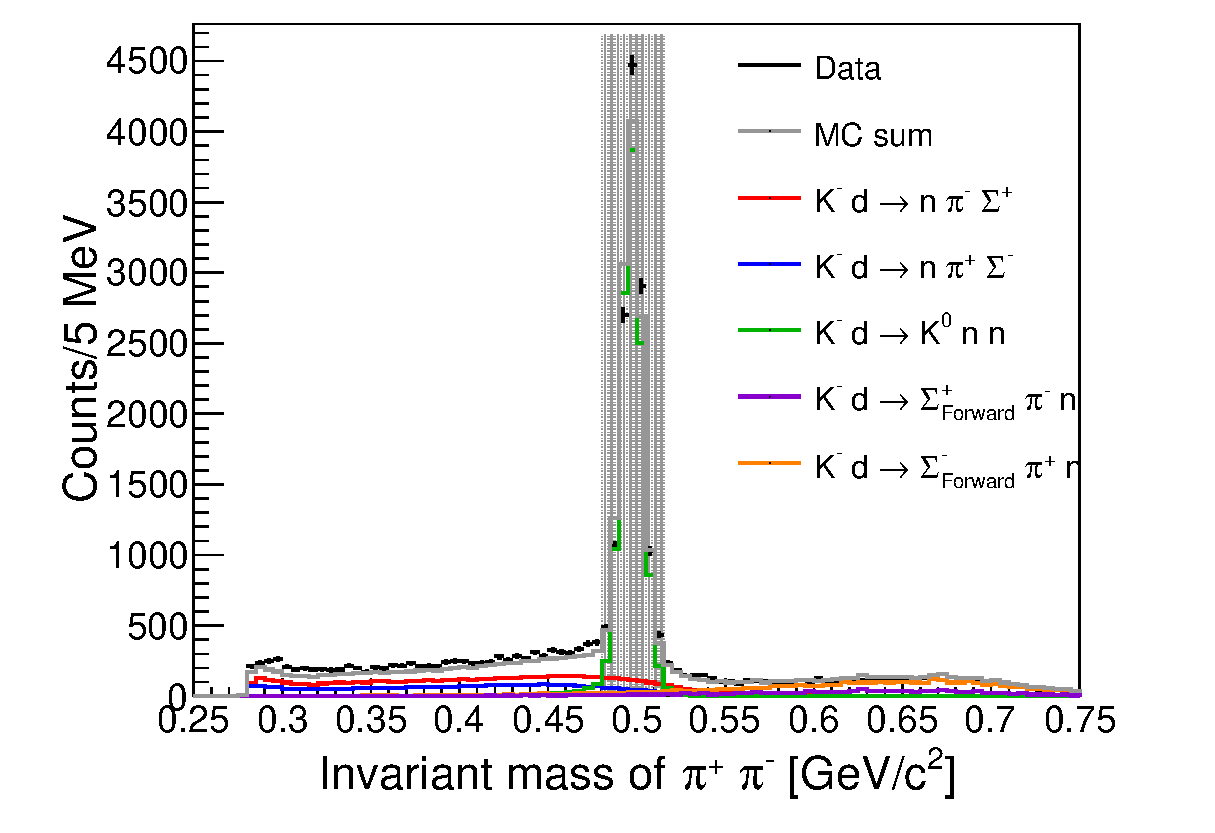
\includegraphics[width=4cm]{../pic/Run78/KN_ana_NC170_25sigma/IM_pipi.eps}
      \end{figure}
    \end{minipage}
    
    \begin{minipage}{0.33\hsize}
      \begin{figure}
        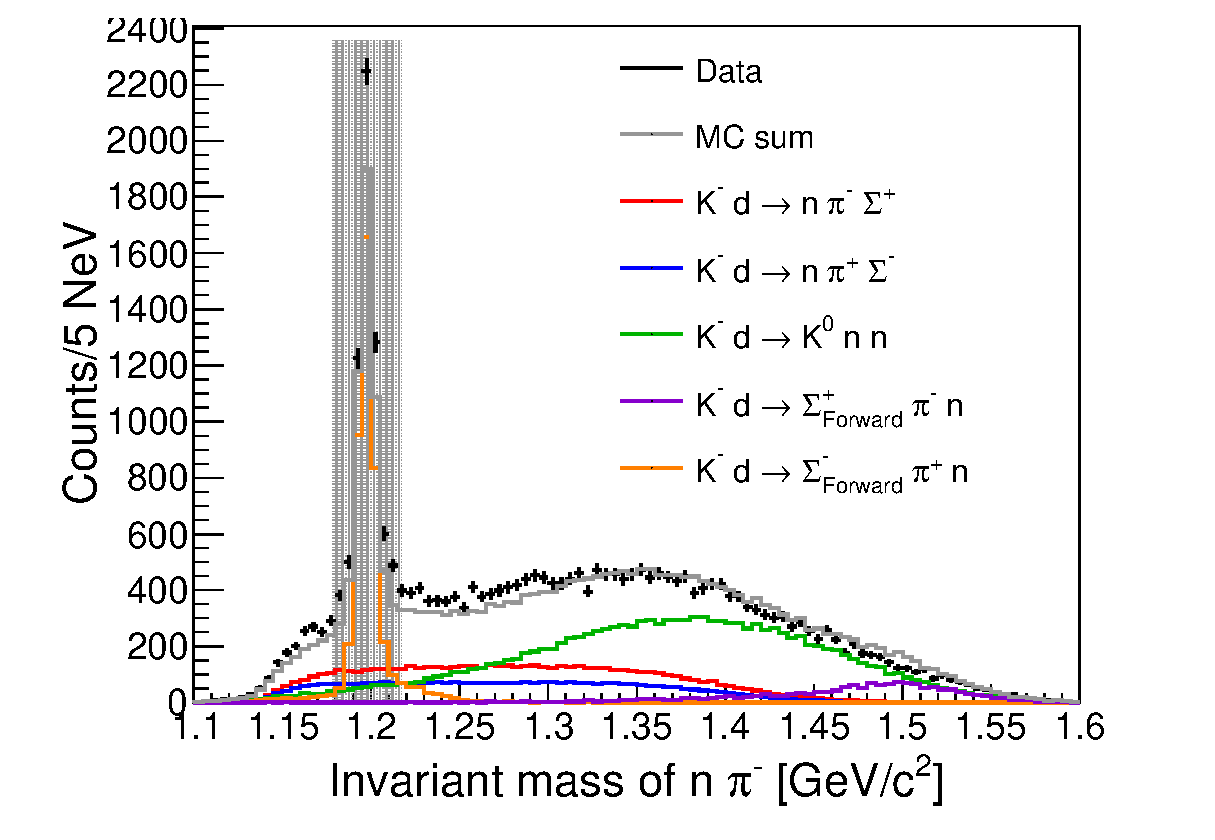
\includegraphics[width=4cm]{../pic/Run78/KN_ana_NC170_25sigma/IM_npim.eps}
      \end{figure}
    \end{minipage}
    
    \begin{minipage}{0.33\hsize}
      \begin{figure}
        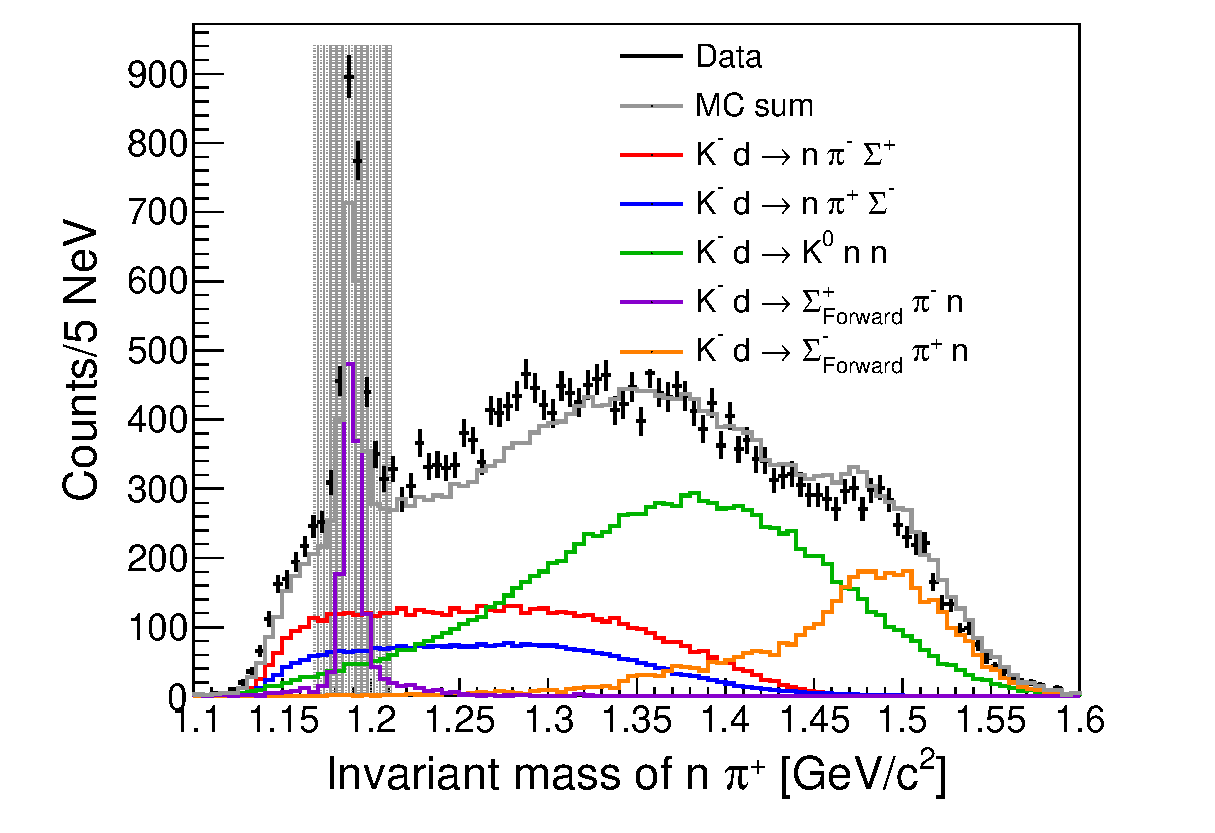
\includegraphics[width=4cm]{../pic/Run78/KN_ana_NC170_25sigma/IM_npip.eps}
      \end{figure}
    \end{minipage}
  \end{tabular}

  %% \begin{tabular}{ccc}
  %%   \begin{minipage}{0.33\hsize}
  %%     \begin{figure}
  %%       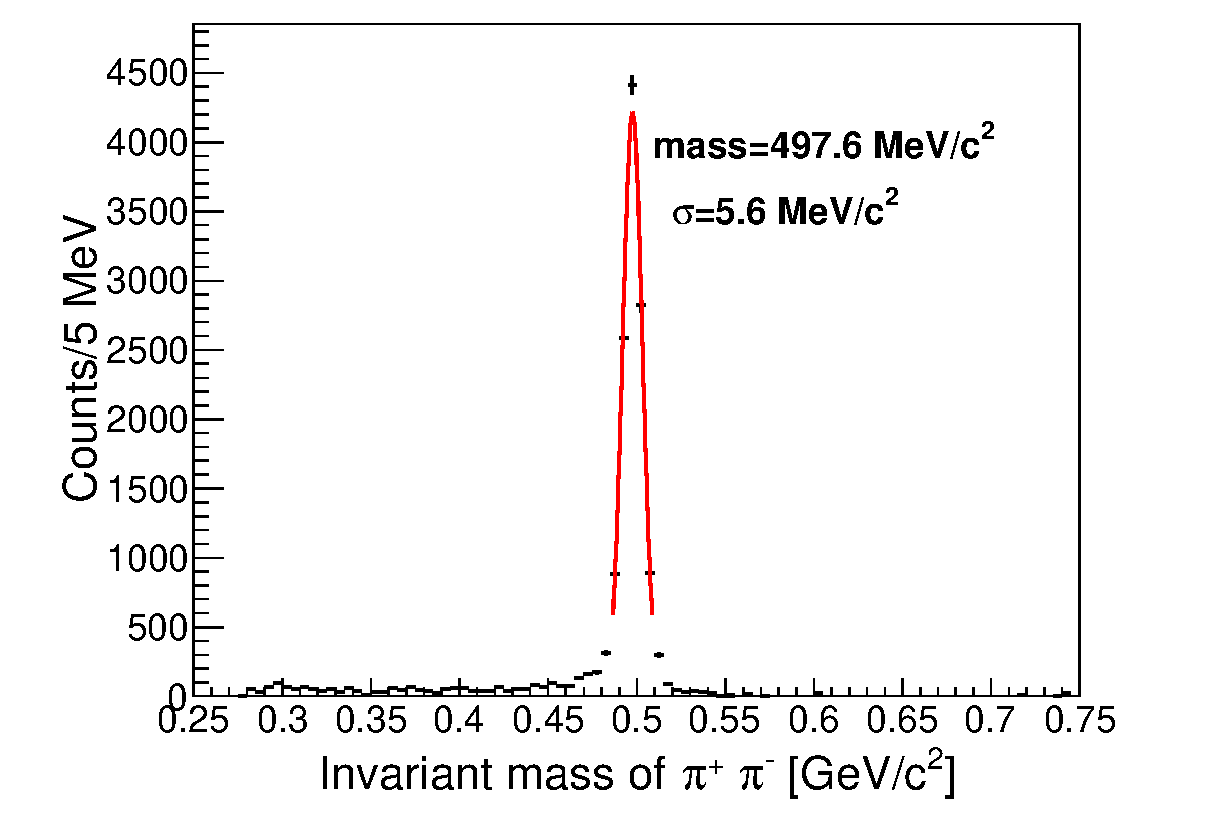
\includegraphics[width=4cm]{../pic/Run78/KN_ana/IM_pipi_fit.eps}
  %%     \end{figure}
  %%   \end{minipage}
    
  %%   \begin{minipage}{0.33\hsize}
  %%     \begin{figure}
  %%       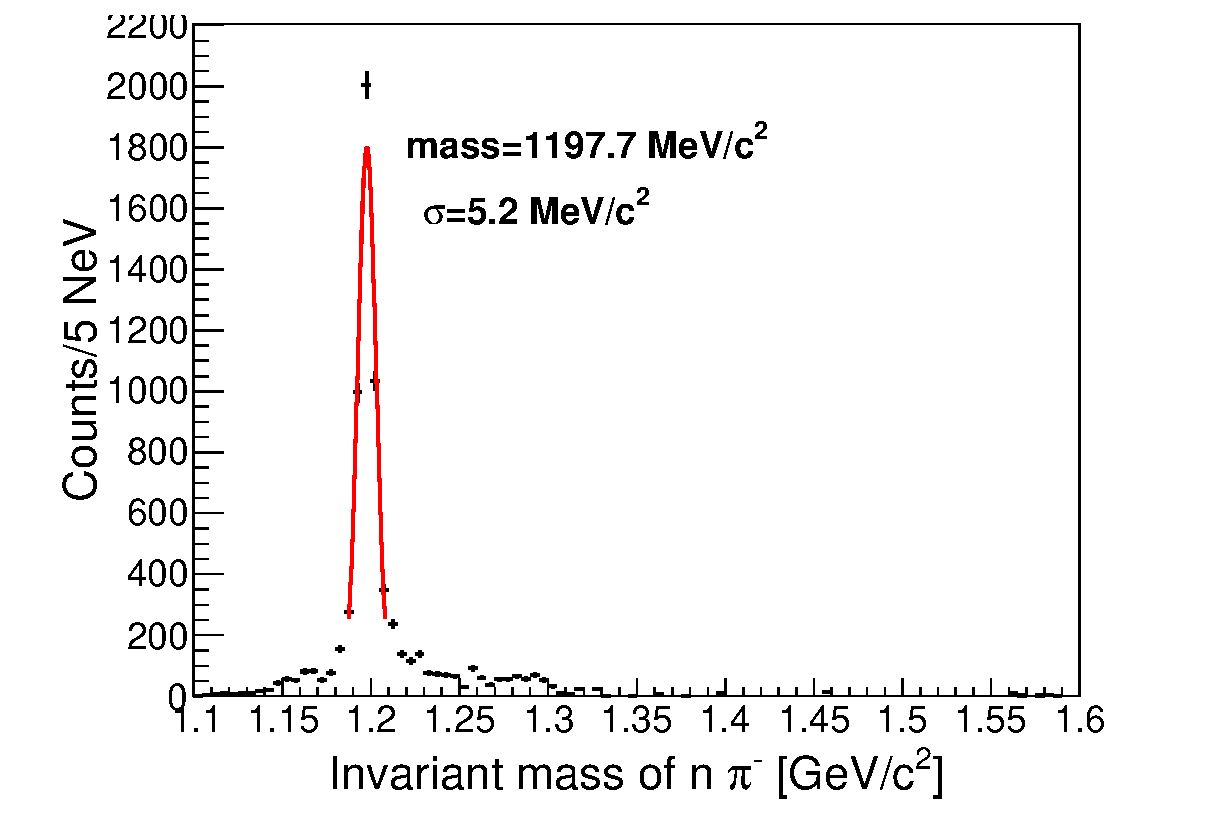
\includegraphics[width=4cm]{../pic/Run78/KN_ana/IM_npim_fit.eps}
  %%     \end{figure}
  %%   \end{minipage}
    
  %%   \begin{minipage}{0.33\hsize}
  %%     \begin{figure}
  %%       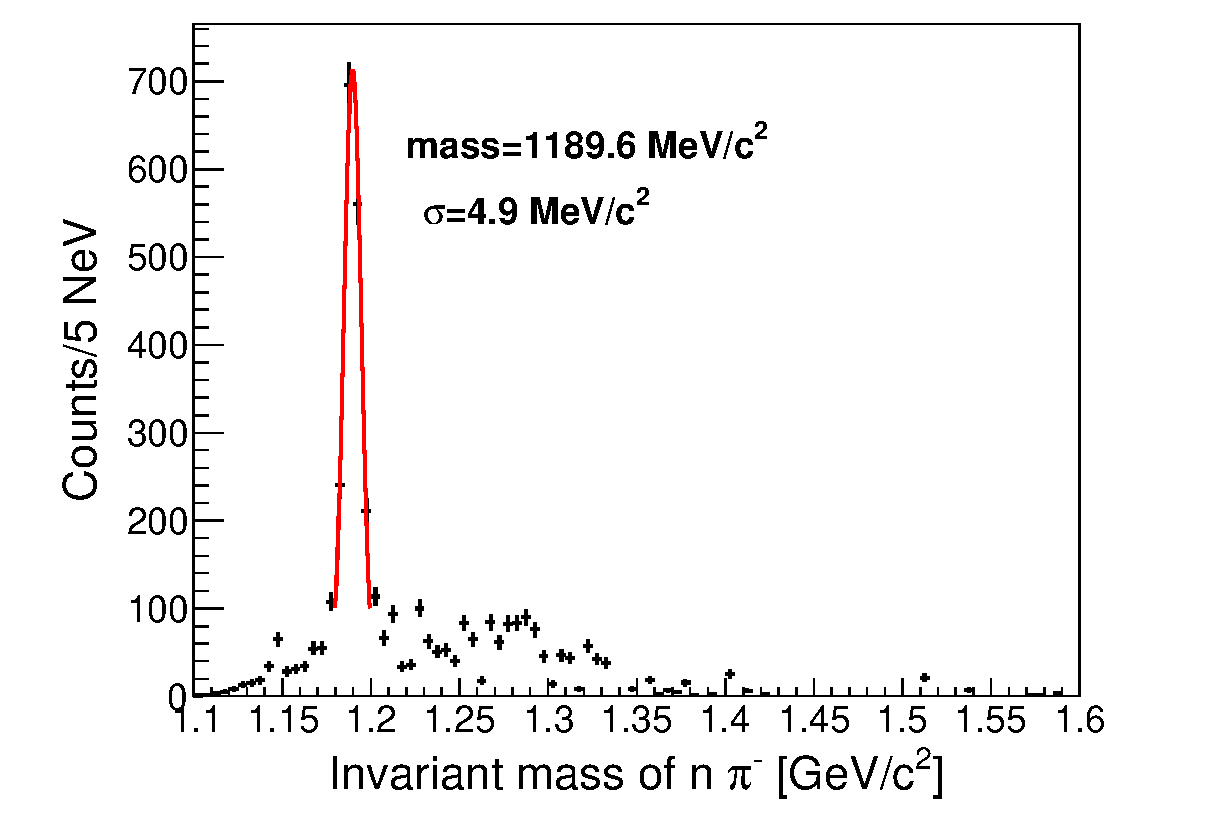
\includegraphics[width=4cm]{../pic/Run78/KN_ana/IM_npip_fit.eps}
  %%     \end{figure}
  %%   \end{minipage}
  %% \end{tabular}
\end{frame}
